\documentclass[a4paper,dvipsnames]{article}

\input ../header
\newcommand{\checkedbox}{\makebox[0pt][l]{$\square$}\raisebox{.15ex}{\hspace{0.1em}$\checkmark$}}
\newcommand{\checkbox}{\makebox[0pt][l]{$\square$}\raisebox{.15ex}{\hspace{0.1em}}\hspace{3mm}}

\begin{document}

\title{Évaluation 5 -- Sujet A}
\author{}
\date{}

\maketitle{}

\pagestyle{empty}

\exo[2 points]\vspace{-2mm} 
Cet exercice est un QCM (questionnaire à choix multiples). Pour chaque question, une seule des réponses proposées est exacte. Entourer la réponse choisie sur le sujet. Aucune justification n'est demandée.

\smallskip

Chaque réponse exacte rapporte $0,5$ point. \textbf{Aucun point n’est enlevé en l’absence de réponse ou en cas de réponse fausse}.

\begin{enumerate}
  \item $\sqrt{18}$ est égal à :
    \begin{multicols}{3}
      \begin{enumerate}
	\item $9$
	\item $2\sqrt{3}$
	\item $3\sqrt{2}$
      \end{enumerate}
    \end{multicols}
  \item Le carré de $3\sqrt{5}$ est :
    \begin{multicols}{3}
      \begin{enumerate}
	\item $15$
	\item $45$
	\item $225$
      \end{enumerate}
    \end{multicols}
  \item On lance une pièce de monnaie truquée pour laquelle \og{}Pile\fg{} sort deux fois plus souvent que \og{}Face\fg{}. On s'intéresse à la face obtenue. La probabilité d'obtenir \og{}Pile\fg{} vaut :
    \begin{multicols}{3}
      \begin{enumerate}
	\item $\dfrac{1}{2}$
	\item $\dfrac{2}{3}$
	\item $\dfrac{1}{3}$
      \end{enumerate}
    \end{multicols}
  \item En Python, le mot-clé qui permet de définir une fonction est :
    \begin{multicols}{3}
      \begin{enumerate}
	\item \mintinline{python}{function}
	\item \mintinline{python}{def}
	\item \mintinline{python}{return}
      \end{enumerate}
    \end{multicols}
\end{enumerate}

\bigskip

\exo[2 points]\vspace{-2mm} Écrire sans racine carrée au dénominateur :
\begin{multicols}{2}
  \begin{enumerate}
    \item $\dfrac{18+\sqrt{2}}{\sqrt{11}}$
    \item $\dfrac{36}{3-\sqrt{2}}\vphantom{\dfrac{\sqrt{2}}{\sqrt{11}}}$
  \end{enumerate}
\end{multicols}
  \dotfill\rep{8}

\bigskip

\exo[1 point]\vspace{-2mm} 
\vspace*{-5mm}
\begin{multicols}{2}
  Lorsqu'on lance une punaise au sol, elle peut se positionner de deux façons : sur le côté (position 1) ou sur la tête (position 2).

  \begin{center}
    
\includegraphics[width=5cm]{evaluation_5_punaise.png}
  \end{center}

  On a effectué $900$ lancers d'une punaise au sol et on a relevé, sur le graphique ci-contre, les fréquences d'apparition de la position $1$ lors de $60$ lancers, $120$ lancers, \dots, jusqu'à $900$ lancers.

  \begin{center}
    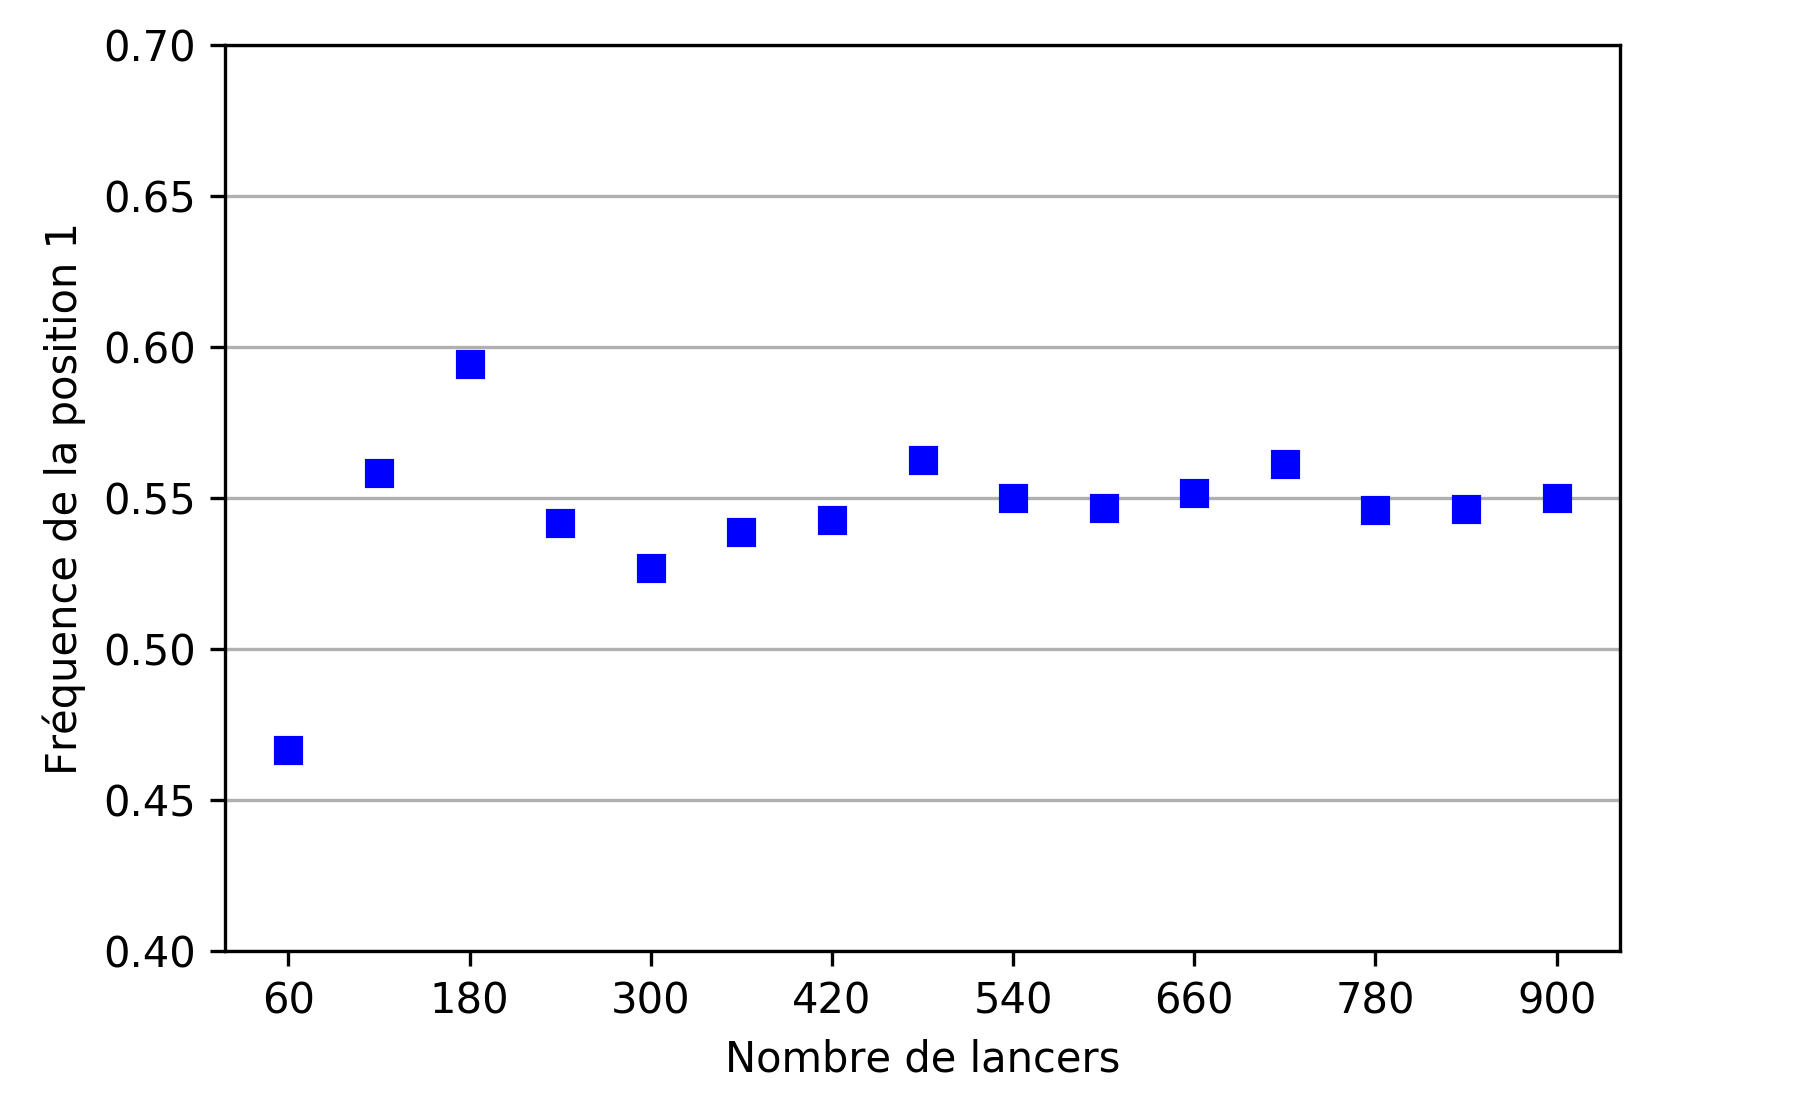
\includegraphics[width=9cm]{evaluation_5_graphique.png}
  \end{center}
\end{multicols}
  Par quelle loi de probabilité semble-t-on pouvoir modéliser cette expérience aléatoire ?\rep{6}

\bigskip

\exo[2 points]\vspace{-2mm} On a écrit chaque lettre du mot \verb|ABRACADABRA| sur un morceau de carton, avant de placer tous les morceaux dans un sac. On choisit ensuite au hasard un morceau de carton dans l'urne, et on note la lettre obtenue.
\begin{enumerate}
  \item Modéliser cette expérience aléatoire.\rep{6}
  \item Quelle est la probabilité d'obtenir une consonne ?\rep{6}
\end{enumerate}

\bigskip

\exo[3 points]\vspace{-2mm} Pour assister aux représentations de danse du mois de juillet, il faut payer $\np{3000}$ XPF par soirée. Cependant, on peut acheter une carte VIP qui coûte $\np{5000}$ XPF et qui permet de ne payer que $\np{2000}$ XPF par soirée.
\begin{enumerate}
  \item On considère la fonction \mintinline{python}{fonction_mystere_1} suivante :
    \begin{minted}{python}
def fonction_mystere_1(n):
    P = 5000 + 2000 * n
    return P
    \end{minted}
   \begin{enumerate}
     \item Que renvoie l'appel \mintinline{python}{fonction_mystere_1(3)} ?\rep{4}
     \item Que représente cette valeur ?\rep{4}
   \end{enumerate} 
 \item Écrire une fonction \mintinline{python}{prix} qui renvoie le prix à payer, sans carte VIP, pour assister à un nombre \mintinline{python}{n} (donné en paramètre de la fonction) de soirées de danse.\rep{8}
\end{enumerate}

\end{document}
